\section{Characterizing Content Delivery Networks by Distributed Active Measurements}\label{sec:aslevel:crowd}

The most popular peer-to-peer overlay network today is Youtube.
Therefore we focus on YouTube.
% motivation
Internet video constitutes more than half of all consumer Internet traffic globally, and its percentage will further increase \cite{ciscovni2013}. Most of the video traffic is delivered by content delivery networks (CDNs). Today the world's largest video CDN is YouTube. Since Google took over YouTube in 2006 the infrastructure of the video delivery platform has grown to be a global content delivery network.
The global expansion of the CDN was also necessary to cope with growing demand of user demands and the high expectations on the video playback. Therefore, content delivery networks try to bring content geographically close to users.
However, the traffic from content delivery networks is highly asymmetric and produces a large amount of costly inter-domain traffic \cite{labovitz2010internet}. Especially Internet Service Providers~(ISPs) providing access to many end users have problems to deal with the huge amount of traffic originating from YouTube. Furthermore, the Google CDN is constantly growing and changing, which makes it difficult for access providers to adapt their infrastructure accordingly.

% problem statement
To understand and monitor the impact of YouTube traffic on ISPs and the topology of CDNs appropriate measurements are aquired. Due to YouTube's load-balancing and caching mechanisms the YouTube video server selection is highly dependent on the location of the measurement points. Hence, we need a globally distributed measurement platform to perform active measurements to uncover the location of YouTube servers. Recent work \cite{adhikari2012vivisecting,adhikari2011you} has performed such measurements in PlanetLab~\cite{planetlab}, a global test bed that provides measurement nodes at universities and research institutes.
The problem is that probes disseminated from PlanetLab nodes origin solely from National Research and Education Networks~(NRENs). This may not reflect the perspective of access ISPs which have a different connection to the YouTube CDN with different peering or transit agreements.

% our methodology
To achieve a better view on the YouTube CDN from the perspective of end users in access networks we use a commercial crowdsourcing platform to recruit regular Internet users as measurement probes.
Thus, we increase the coverage of vantage points for the distributed measurement of the YouTube CDN.
To evaluate the impact of the measurement platform and the coverage of their vantage point,  we perform the same measurements using PlanetLab nodes and crowdsourcing users and compare the obtained results.

% our contribution
Our measurements show that distributed measurements in PlanetLab are not capable to capture a globally distributed network, since the PlanetLab nodes are located in NRENs where the view on the Internet is limited. We demonstrate that recruiting users via crowdsourcing platforms as measurement probes can offer a complementary view on the Internet, since they provide access to real end users devices located out side of these dedicated research networks.
This complementary view can help to gain a better understanding of the characteristics of Video CDNs.
Concepts like ALTO or economic traffic management (ETM) \cite{bookchapter2009-12} need a global view of the CDN structure to optimize traffic beyond the borders of ISPs.
%what in turn  might have implications for network operators in mechanism design and resource provisioning.
Finally, models for simulation and performance evaluation of mechanisms incorporating CDNs need to apply the characteristics identified by crowd sourced network measurements.
%In this work, we propose a new measurement methodology which benefits of the distribution of crowdsourcing workers on internet access provider networks.

% structure
The measurements conducted in the PlanetLab and via crowdsourcing are described in Section~\ref{sec:method}.
In Section~\ref{sec:results} we provide details on the measurement results and their importance for the design of distributed network measurements.

% todo matthias
test

\subsection{Distributed Active Measurement Description}
\label{sec:method}

To assess the capability of crowdsourcing for distributed active measurements we conduct measurements with both  PlanetLab and the commercial Crowdsourcing platform Microworkers~\cite{microworkers}.
We measure the global expansion of the YouTube CDN by resolving physical server IP-addresses for clients in different locations.

\subsubsection{Description of the PlanetLab Measurement}

PlanetLab is a publicly available test bed, which currently consists of 1173 nodes at 561 sites.
The sites are usually located at universities or research institutes.
Hence, they are connected to the Internet via NRENs.
To conduct a measurement in PlanetLab a slice has to be set up which consists of a set of virtual machines running on different nodes in the PlanetLab test bed.
Researchers can then access these slides to install measurement scripts.
In our case the measurement script implemented in Java extracted the server hostnames of the page of three predetermined YouTube videos and resolved the IP addresses of the physical video servers.
The IP addresses of the PlanetLab clients and the resolved IP addresses of the physical video servers were stored in a database.
To be able to investigate locality in the YouTube CDN, the geo-location of servers and clients is necessary.
For that purpose the IP addresses were mapped to geographic coordinates with MaxMinds GeoIP database \cite{geolite}.
The measurement was conducted on 220 randomly chosen PlanetLab nodes in March 2012.

\subsubsection{Description of the Crowdsourcing Measurement}
To measure the topology of the YouTube CDN from an end users point of view who is connected by an ISP network we used the crowdsourcing platform Microworker~\cite{microworkers}.
The workers were asked to access a web page with an embedded Java application, which automatically conducts client side measurements.
These include, among others, the extraction of the default and fallback server URLs from three predetermined YouTube video pages.
The extracted URLs were resolved to the physical IP address of the video servers locally on the clients.
The IP addresses of video servers and of the workers client were sent to a server which collected all measurements and stored them in a database.

In a first measurement run, in December 2011, 60 different users of Microworkers participated in the measurements.
Previous evaluation have shown, that the majority of the platform users is located in Asia~\cite{conf2011-410}, and accordingly most of the participants of there first campaign were from Bangladesh.
In order to obtain wide measurement coverage the number of Asian workers participating in a second measurement campaign, conducted in March 2012, was restricted.
In total, 247 workers from 32 different countries, finished the measurements successfully identifying 1592 unique physical YouTube server IP addresses.

%\subsection{Model Validation}
\subsection{Numerical Examples}\label{sec:hierarchical:analyticbw:results}

We evaluate the performance of tiered caching systems with bandwidth constraints in parameter studies.
We validate the model via simulations, which allows us to verify the accuracy of the analytical model and the validity of our conclusions based on the model for a wide range of system parameters.
Before presenting numerical examples, we briefly describe the event-based simulation.
%We compare the results derived from our analytical models with results derived by event-based simulation.
The simulation framework used is implemented in Matlab and described in detail in \cite{info3-inproceedings-2015-530}. The results presented show the mean values of 8 runs with 95\% confidence intervals, each run simulating $10^5$ requests in the stationary phase.

If not stated otherwise, in the remainder of this study, the catalogue size is $N=1e6$.
The number of tier-1 caches is $n_1=1e4$, each having a capacity of $C_1=8$.
There is one tier-2 cache with default capacity $C_2=1e4$.
The tier-1 cache upload bandwidth is limited to $0.8\text{Mbps}$, whereas the tier-2 cache has unlimited upload bandwidth.

\begin{figure*}[!tb]
\begin{minipage}[t]{\textwidth}
  \centering
  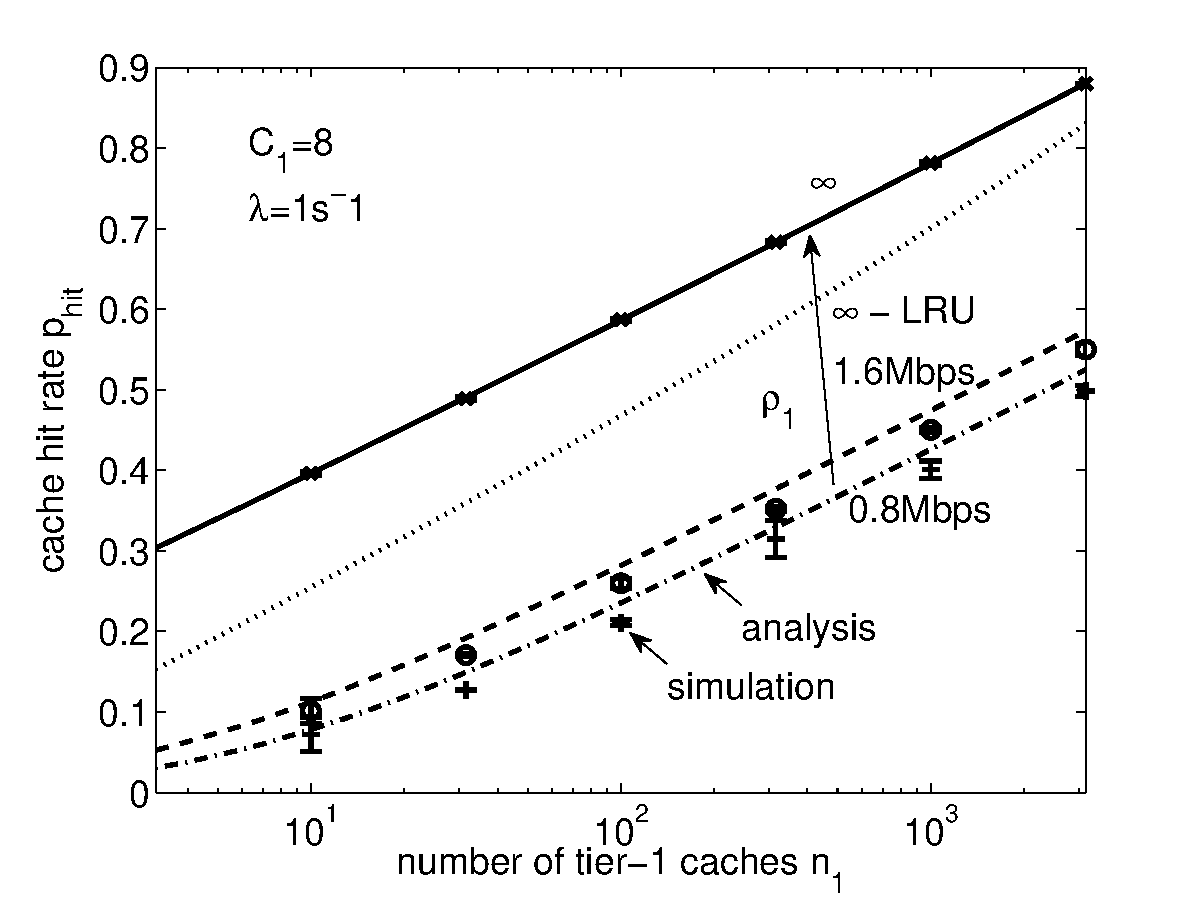
\includegraphics[width=0.7\textwidth]{hierarchical/analyticbw/figures/hwc_CISP0}
  \caption{Comparison of cache hit rate for optimal placement with LRU policy.}
  \label{fig:hwc_CISP0}
\end{minipage}
%\hspace{0.01\textwidth}
\begin{minipage}[t]{\textwidth}
  \centering
  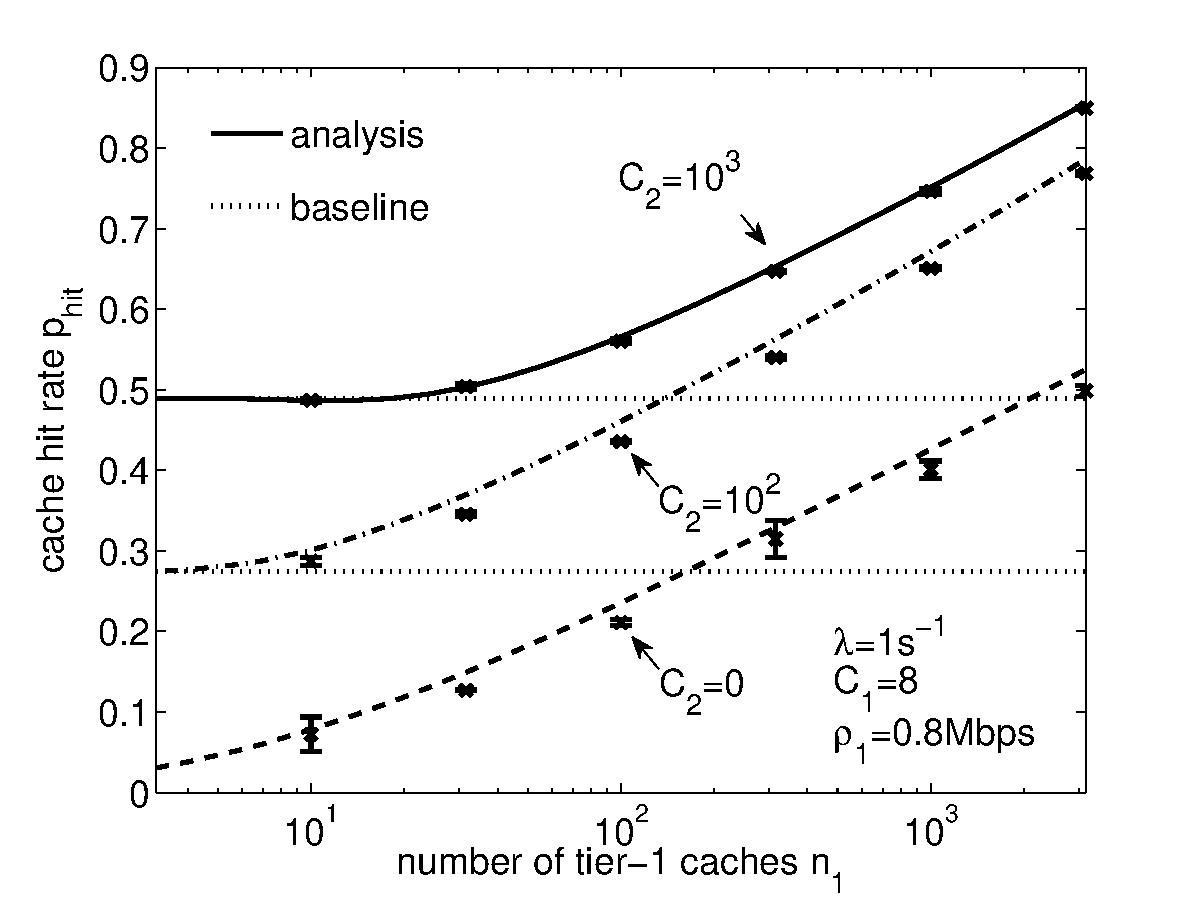
\includegraphics[width=0.7\textwidth]{hierarchical/analyticbw/figures/hwc_l1C8_C2}
  \caption{Cache hit rate dependent on the number of tier-1 caches for different tier-2 cache capacities.}
  \label{fig:hwc_l1C8_C2}
\end{minipage}
% \hspace{0.01\textwidth}
% \begin{minipage}[b]{0.32\textwidth}
%   \centering
%   \includegraphics[width=1\textwidth]{hierarchical/analyticbw/figures/hwc_C8C1e3_l0}
%   \caption{Cache hit rate dependent on the number of tier-1 caches for varying request rates $\lambda$.}
%   \label{fig:hwc_C8C1e3_l}
% \end{minipage}
\end{figure*}

%\begin{itemize}
%	\item Methodology
%	\item Performance metrics \\
%    - cache capacity of ISP cache necessary to replace home routers
%	\item Results
%  \item upper bound wrt uploadrate optimal case, always hit in tier 2
%  \item Optimal strat dependent on AS size and HG capacity
%  \item Optimization -> LCP with P ~ overlay distribution
%   \item request rate proportional AS size -> HWC
%\end{itemize}

% \begin{figure}[tb]
%   \centering
%   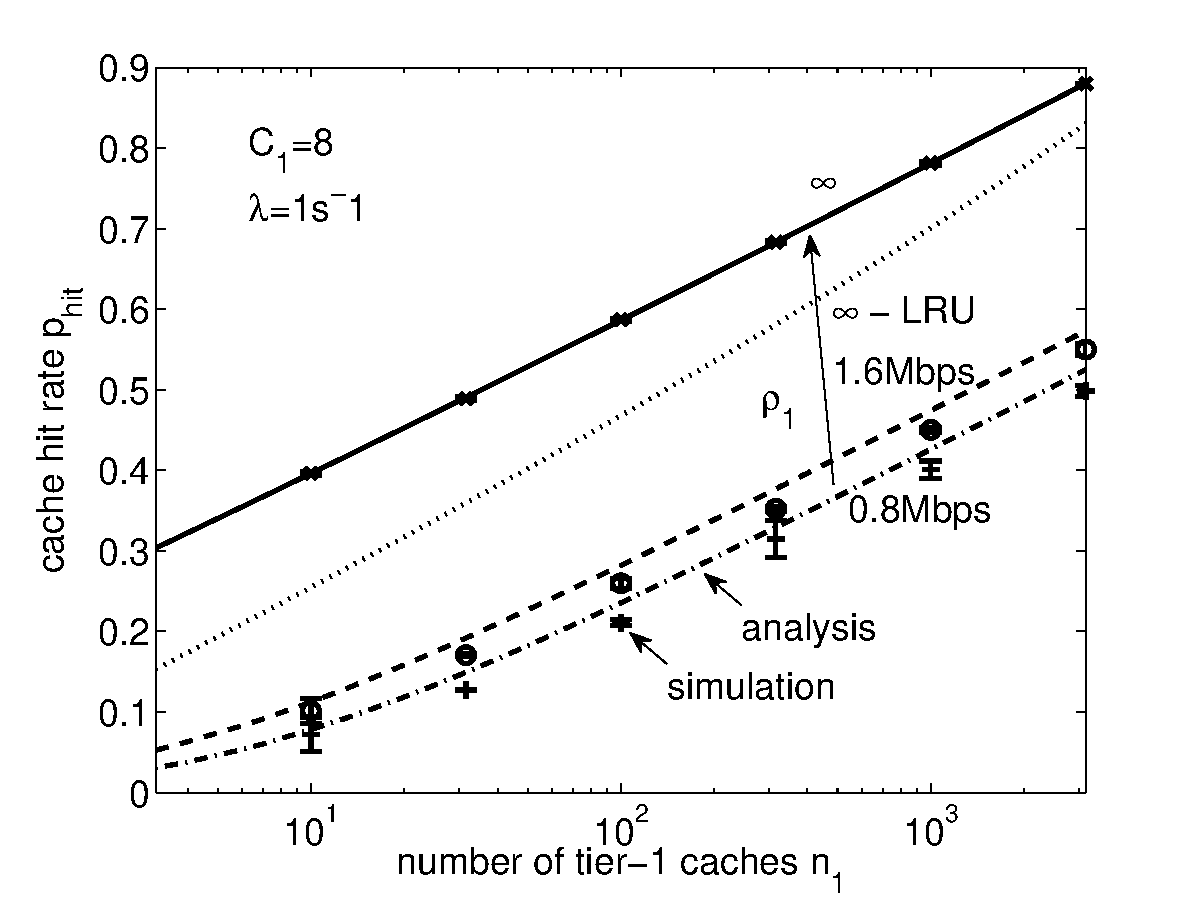
\includegraphics[width=0.7\textwidth]{hierarchical/analyticbw/figures/hwc_CISP0}
%   \caption{Comparison of cache hit rate for optimal placement with LRU policy.}
%   \label{fig:hwc_CISP0}
% \end{figure}
%
% \begin{figure}[tb]
%   \centering
%   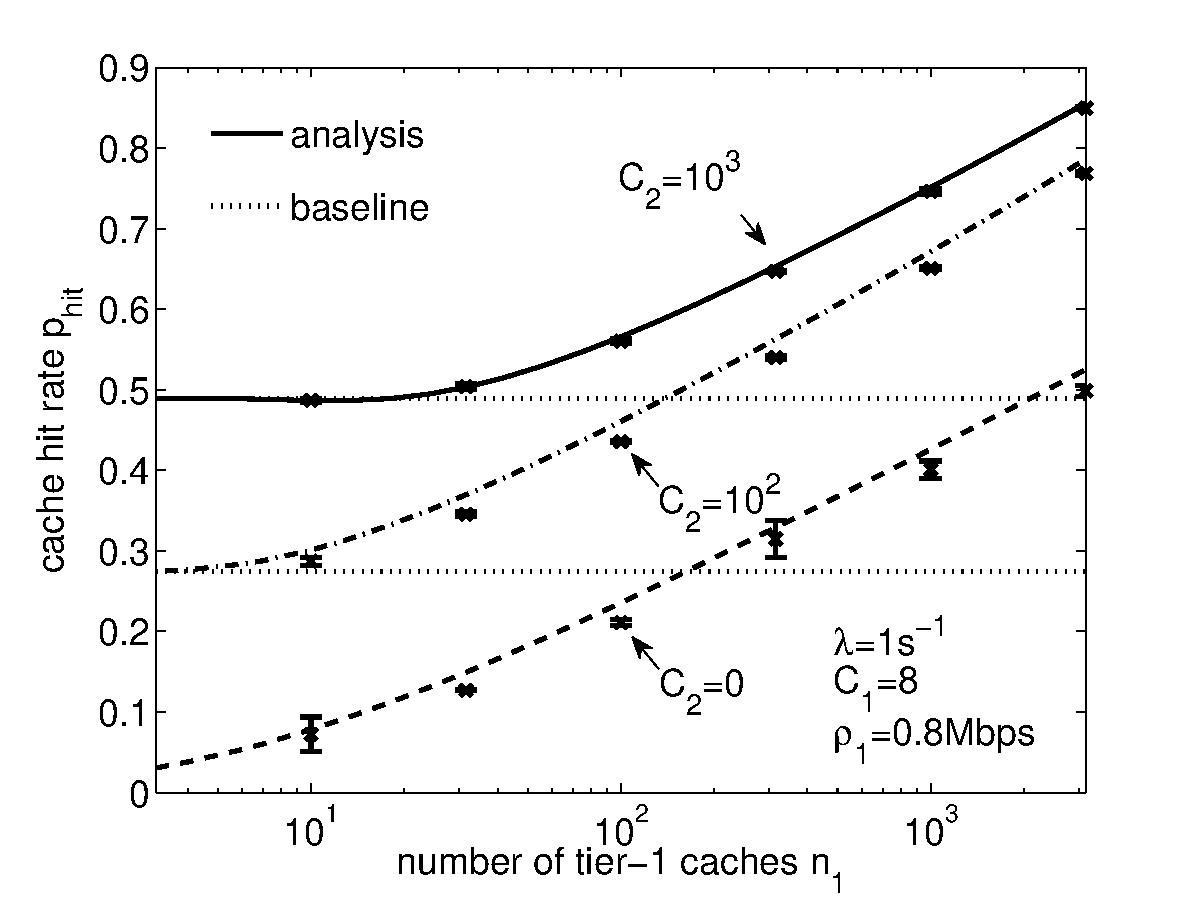
\includegraphics[width=0.7\textwidth]{hierarchical/analyticbw/figures/hwc_l1C8_C2}
%   \caption{Cache hit rate dependent on the number of tier-1 caches for different tier-2 cache capacities.}
%   \label{fig:hwc_l1C8_C2}
% \end{figure}

% \begin{figure}[tb]
% \centering
% 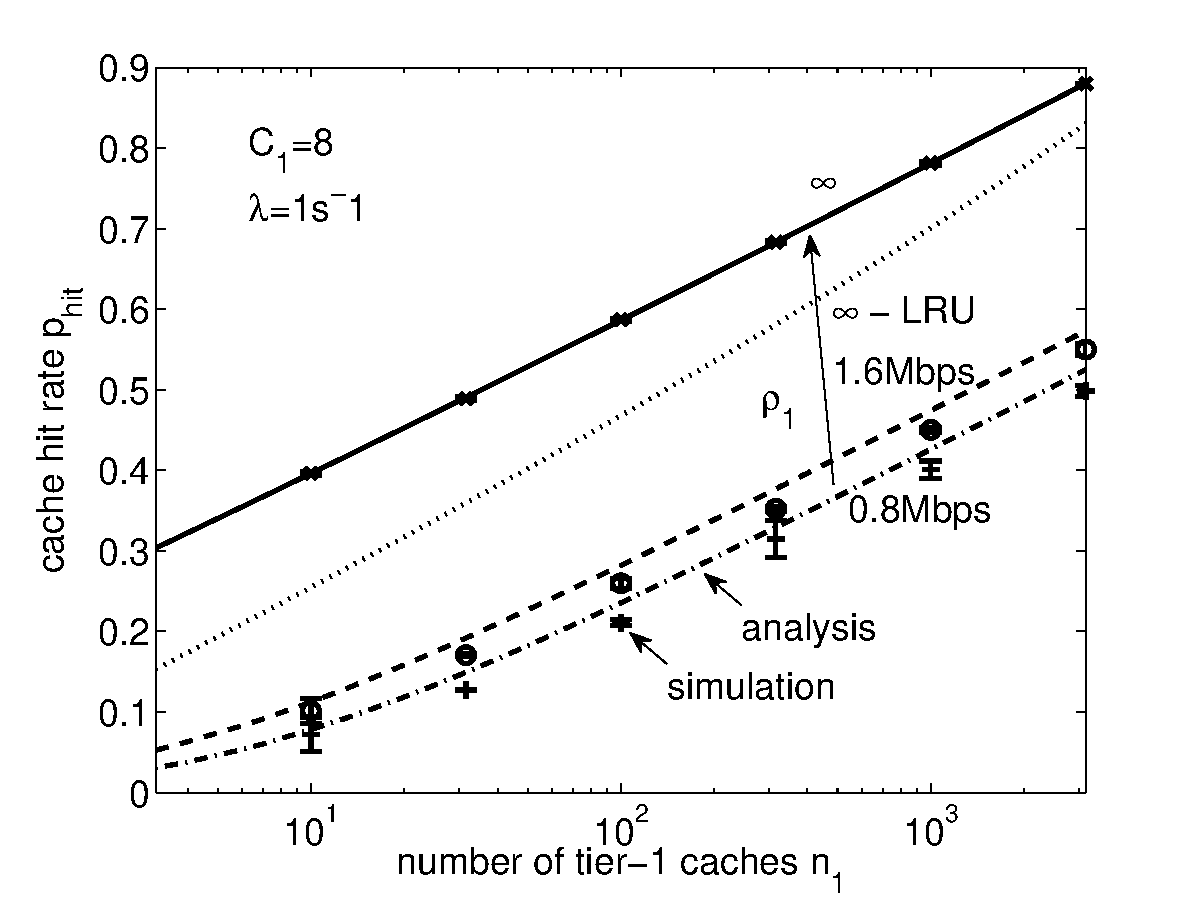
\includegraphics[width=75mm]{hierarchical/analyticbw/figures/hwc_CISP0}
% \caption{Cache hit rate dependent on number of tier-1 caches. Comparison of optimal placement with LRU policy.}
% \label{fig:hwc_CISP0}
% \end{figure}
% \begin{figure}[tb]
% \centering
% 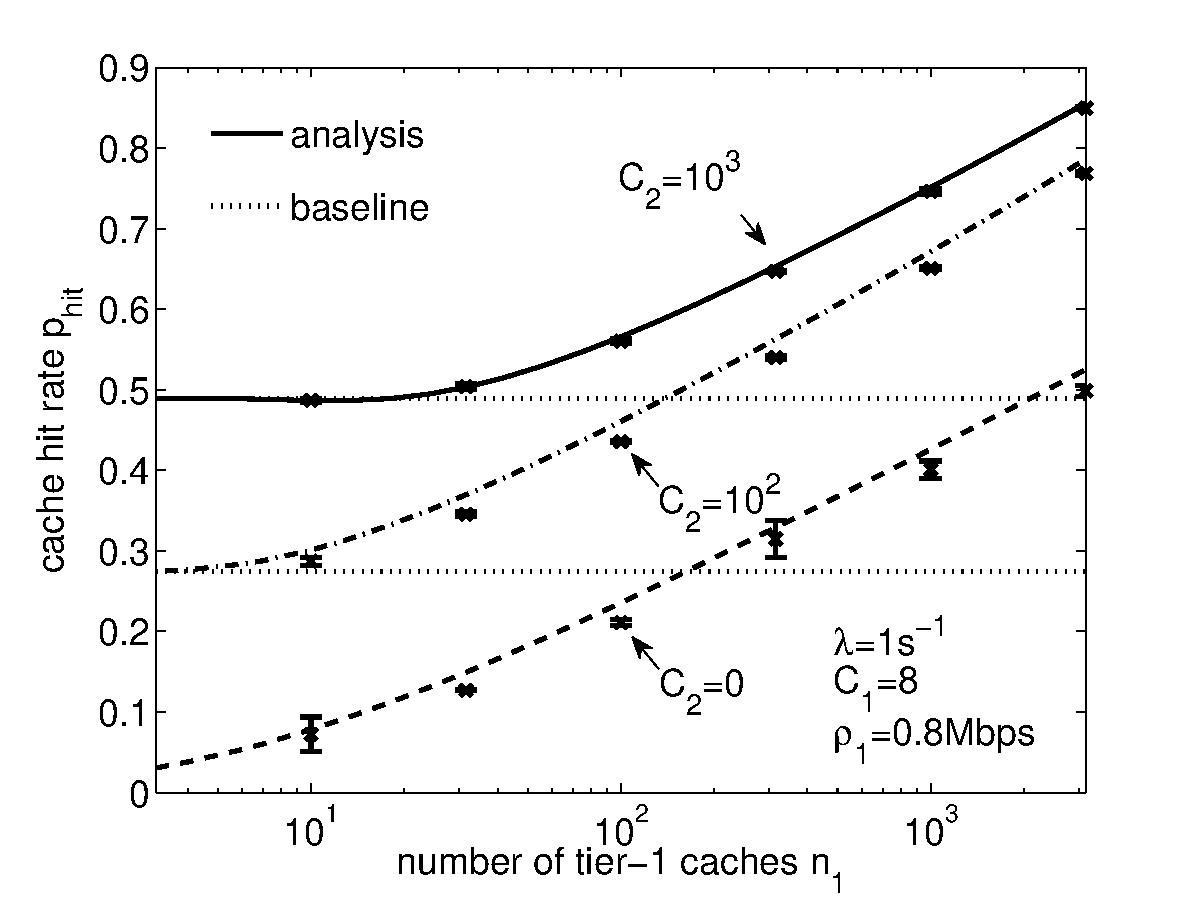
\includegraphics[width=75mm]{hierarchical/analyticbw/figures/hwc_l1C8_C2}
% \caption{Cache hit rate dependent on the number of tier-1 caches for different tier-2 cache capacities.}
% \label{fig:hwc_l1C8_C2}
% \end{figure}
% \begin{figure}[tb]
% \centering
% \includegraphics[width=75mm]{hierarchical/analyticbw/figures/hwc_C8C1e3_l0}
% \caption{Cache hit rate dependent on the number of tier-1 caches for varying request rates $\lambda$.}
% \label{fig:hwc_C8C1e3_l}
% \end{figure}

\begin{figure}[tb]
  \centering
  \includegraphics[width=0.7\textwidth]{hierarchical/analyticbw/figures/hwc_C8C1e3_l0}
  \caption{Cache hit rate dependent on the number of tier-1 caches for varying request rates $\lambda$.}
  \label{fig:hwc_C8C1e3_l}
\end{figure}

\begin{figure}[tb]
  \centering
  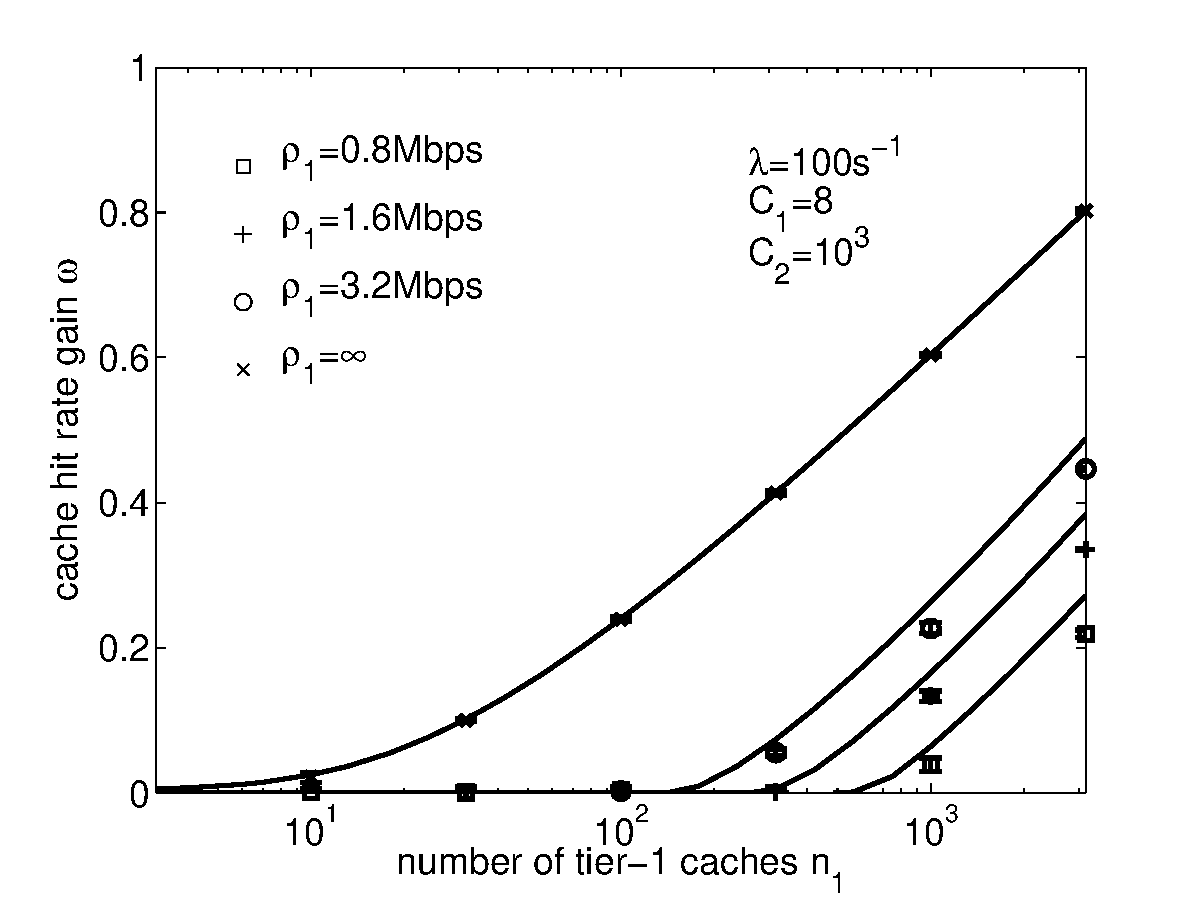
\includegraphics[width=0.7\textwidth]{hierarchical/analyticbw/figures/hwc_C8l100_gain}
  \caption{Impact of the upload bandwidth $\rho_1$ on the cache hit rate gain $\omega$.}
  \label{fig:hwc_C8l100_gain}
\end{figure}

% \begin{figure*}[bt]
% \begin{minipage}[t]{0.49\textwidth}
%   \centering
%   \includegraphics[width=\textwidth]{hierarchical/analyticbw/figures/hwc_C8C1e3_l0}
%   \caption{Cache hit rate dependent on the number of tier-1 caches for varying request rates $\lambda$.}
%   \label{fig:hwc_C8C1e3_l}
% \end{minipage}
% \hspace{0.01\textwidth}
% \begin{minipage}[t]{0.49\textwidth}
%   \centering
%   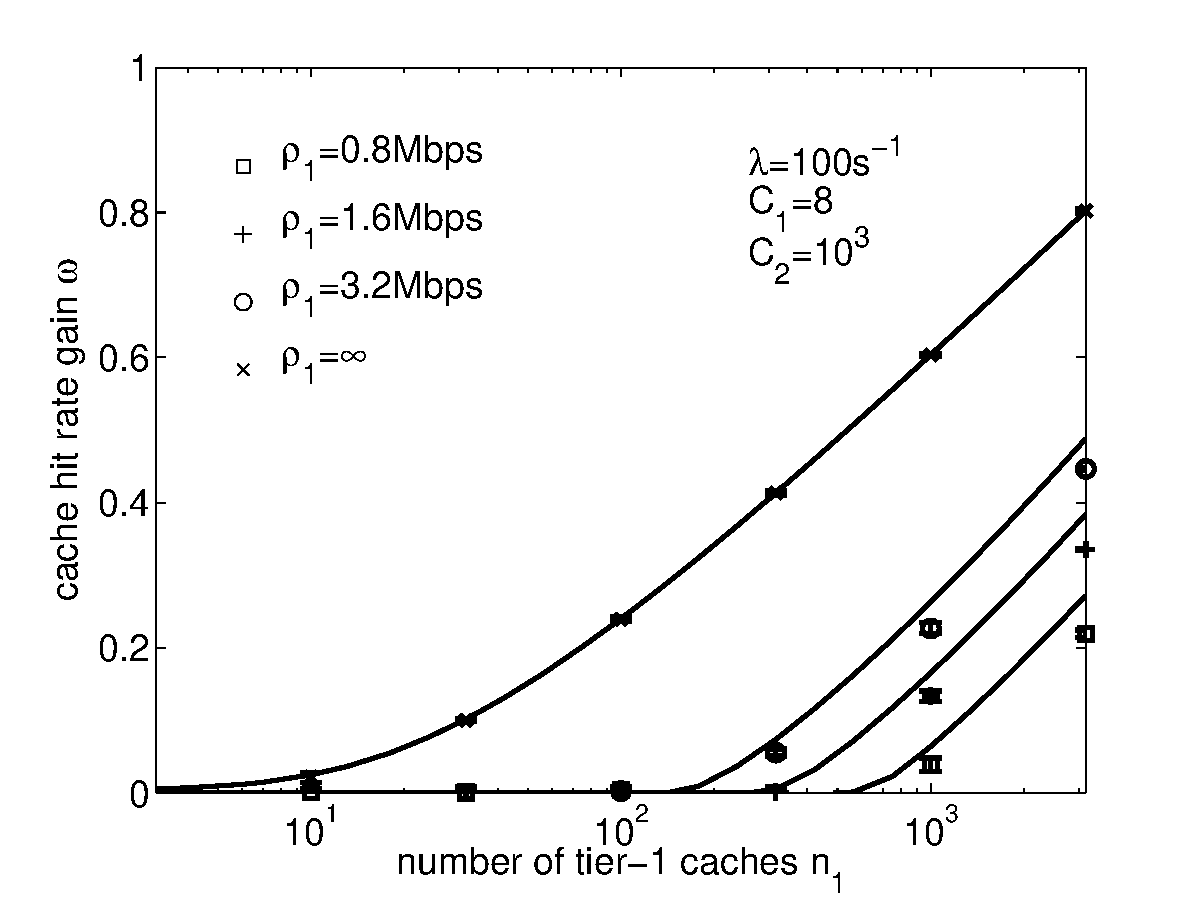
\includegraphics[width=\textwidth]{hierarchical/analyticbw/figures/hwc_C8l100_gain}
%   \caption{Impact of the upload bandwidth $\rho_1$ on the cache hit rate gain $\omega$.}
%   \label{fig:hwc_C8l100_gain}
%   \end{minipage}
% \end{figure*}

We first consider a scenario without tier-2 cache.
In this case the caching architecture only consists of tier-1 caches.
We evaluate the cache hit rate dependent on the number of tier-1 caches $n_1$.
Figure~\ref{fig:hwc_CISP0} shows the results for different upload bandwidth of tier-1 caches $\rho_1$.
The cache hit rate increases with the number of tier-1 caches and their upload bandwidth.
The analytic model slightly overestimates the cache hit rate for finite upload bandwidth of tier-1 caches.
In the case of infinite upload bandwidth, the results can be compared to an LRU cache with capacity $n_1 C_1$.
In the optimal placement, the items that are most frequently requested are placed on the caches, which explains the higher hit rate compared to LRU.
Hence, there is a high potential to increase the hit rate of the system by using an optimal content placement used.
Furthermore, the results show that it is important to consider bandwidth constraints in the analysis of caching systems.
If the bandwidth is limited to 1.6Mbps, the cache hit is reduced by about 30\% compared to the case of unlimited bandwidth.

% \begin{figure}[tb]
% \centering
% \includegraphics[width=75mm]{figures/hwc_C8C1e3_l0}
% \caption{Cache hit rate dependent on the number of tier-1 caches for varying request rates $\lambda$.}
% \label{fig:hwc_C8C1e3_l}
% \end{figure}

% \begin{figure}[tb]
% \centering
% 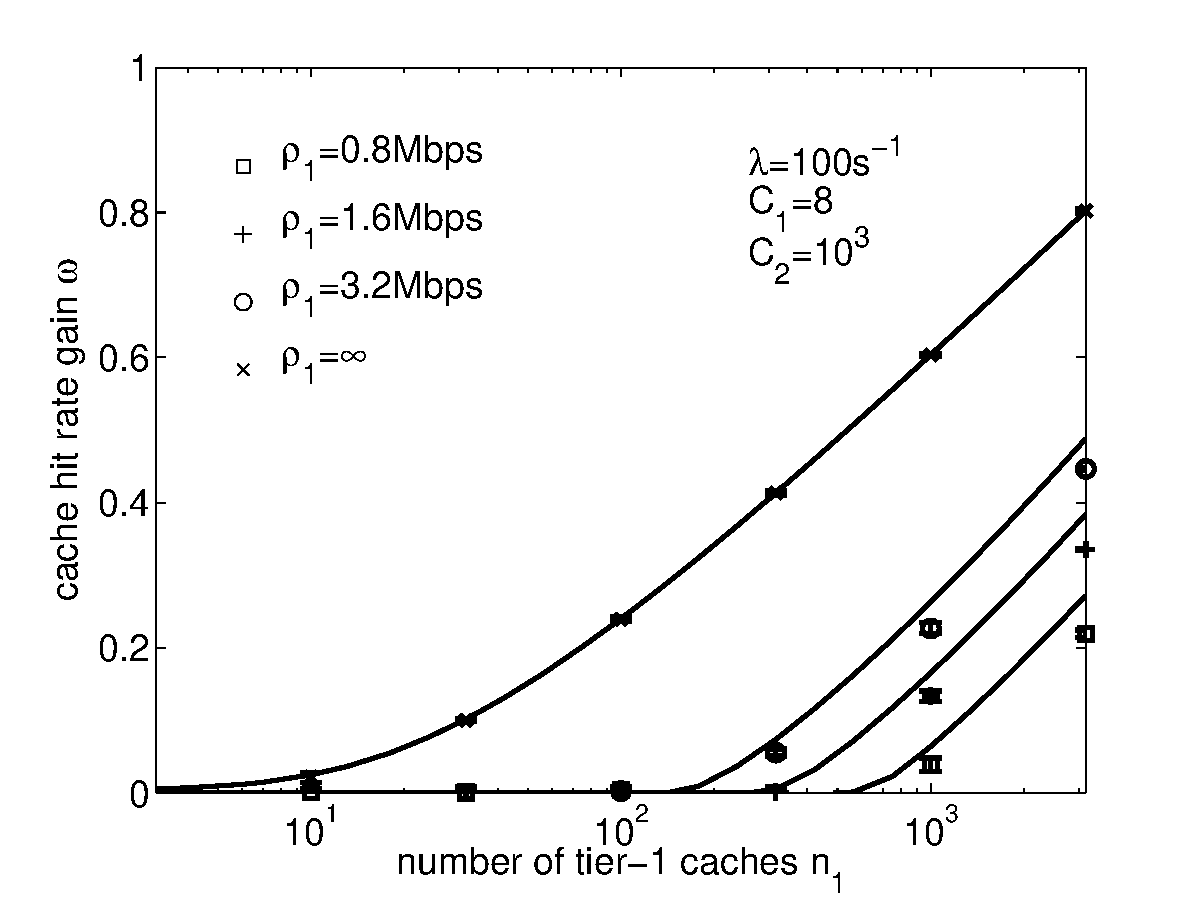
\includegraphics[width=70mm]{hierarchical/analyticbw/figures/hwc_C8l100_gain}
% \caption{Impact of the upload bandwidth $\rho_1$ on the cache hit rate gain $\omega$.}
% \label{fig:hwc_C8l100_gain}
% \end{figure}

To investigate the influence of the tier-2 cache on the cache hit rate, we vary the tier-2 cache capacity $C_2$.
Figure~\ref{fig:hwc_l1C8_C2} depicts the hit rate of the tiered caching architecture dependent on the number of tier-1 caches for different tier-2 cache capacities.
As baselines the cache hit rate $p'_\text{hit}(2)$ of a single tier-2 cache with capacity $C_2$ without tier-1 support is depicted.
The overall hit rate increases with the tier-2 cache capacity.
%If a high tier-2 cache capacity is available the number of tier-1 caches necessary to increase the performance of the tiered caching architecture is higher.

The performance of the caching architecture also highly depends on the overall request rate $\lambda$.
Figure~\ref{fig:hwc_C8C1e3_l} shows the cache hit rate dependent on the number of tier-1 caches for varying request rates $\lambda$.
Due to the limited upload bandwidth of tier-1 caches, more requests are blocked and forwarded to the tier-2 cache, which reduces the total rate of requests hit and served by tier-1 and tier-2 caches.
If the request rate increases, more tier-1 caches are necessary to increase the overall hit rate.
%For a rate of 100 requests per second, $10^3$ tier-1 caches are necessary to slightly increase the hit rate in this case.

In order to evaluate the performance of the tiered caching architecture for a medium sized ISP, we consider a high request rate $\lambda=100s^{-1}$ and a high tier-2 cache capacity $C_2=10^3$.
We study the impact of the upload bandwidth of tier-1 caches on the cache hit rate gain $\omega$.
If the upload bandwidth of the caches is low, a high number of tier-1 caches is necessary to improve the performance of the caching architecture.
The number of tier-1 caches necessary to gain hit rate decreases with their upload bandwidth.

Hence, if no tier-2 cache or only a small tier-2 cache is available, the system benefit depends on the number and bandwidth of tier-1 caches available.
In larger ISPs where a large tier-2 cache is available and where the request rate of items is high, the approach is only beneficial if the number or upload bandwidth of tier-1 caches is high enough.

%\begin{figure}[tb]
%\centering
%\includegraphics[width=75mm]{figures/ana_sim_all}
%\caption{TODO AS-Rank}
%\label{fig:ana_sim_all}
%\end{figure}

